%\section{Systems for experiments}
\section{Supercomputing Systems}
\label{sec:systems}

In this section, we describe the BG/Q resources at the Argonne Leadership Computing Facility (ALCF) on which we developed and tested our multipath sparse data movement algorithms.

ACLF maintains several compute analysis systems that are used by the scientific community. Figure \ref{fig:alcf} depicts the architecture of ALCF’s primary resource, Mira, its data analysis cluster, Tukey, and the file server nodes.

\begin{figure}[!htb]
\vspace{-0.1in}
\centering
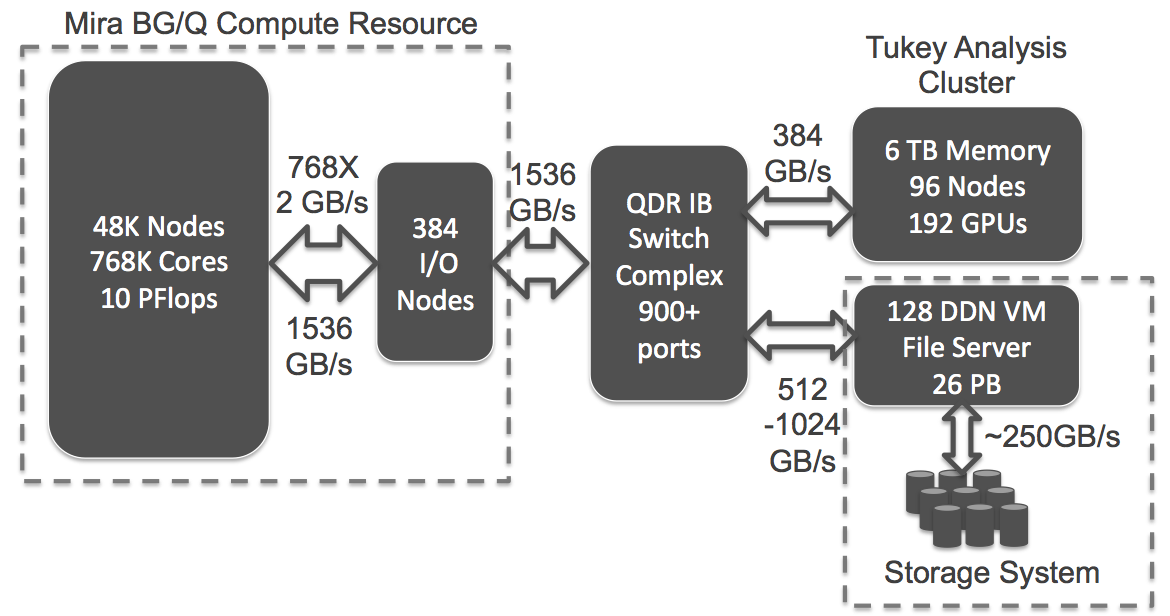
\includegraphics[scale=0.2]{figures/anl_facility}
\vspace{-0.1in}
\caption{The ALCF maintains the 768K core Blue Gene/Q supercomputer (Mira), data analysis cluster (Tukey), and file server nodes.}
\vspace{-0.1in}
\label{fig:alcf}
\end{figure}

Mira has 48K nodes and has a peak performance of 10 petaflops. Each node has 16 application cores and 16 GB of memory.
Mira’s I/O and interprocessor communications (both point-to-point and collectives) travel on a 5D torus network. This 5D torus interconnects each compute node with its 10 neighbors at 2 GB/s theoretical peak over each link in each direction, making a total of 40 GB/s bandwidth in both directions for one single compute node. However, due to packet and protocol overheads, up to 90\% of the raw data rate (1.8GB/s) is available for user data. The machine can be partitioned into non-overlapping rectangular sub-machines for certain applications upon request. These sub-machines do not interfere with each other except for I/O nodes and the corresponding storage system.

An overview of the network is also given in \cite{Chen:MessagingUnit}. Each compute node has 11 send units and 11 receive units (10 for the links of the torus and one for the I/O link). All packets are injected in and pulled out of network injection/reception FIFOs by Messaging Unit (MU). The number of FIFOs is enough to saturate all links. Outgoing packets can be put in any injection FIFOs and may go out to any link. However, incoming packets at a receiver is placed only in its reception FIFO.

For interconnect network traffic, the BG/Q supports both deterministic and dynamic routing \cite{Chen:BGQ}. Deterministic routing uses only one path to route packets from a source to a destination and packets are routed longest to shortest using a commonly used dimension-order routing algorithm. In dynamic routing, routing is still dimension ordered, but the packet routes are programmable, enabling different routing algorithms to be used. This is called ``zone routing''. There are four zone IDs from 0 to 3. The routing algorithm selects a zone ID based on a flexibility metric and the message size. The flexibility value is computed based on the torus size and hop distance between the two communicating nodes. The selection of zone ID based on these values is experiment-based and is hard coded in low-level libraries \cite{BGQRedbook:Gilge}. Among the four routing zones, routing zone ID 1 is unrestricted, and packets route in a random order. Routing zone ID 0 is longest-to-shortest. However, dimensions with the same lengths can be chosen randomly. Routing zone IDs 2 and 3 are deterministic. For these two routing zone IDs, given a certain message size, routing is always the same and its path is known before it is routed. These are default routing algorithms and are not changeable. However, we can set a routing zone ID by using a PAMI ROUTING environment variable. As BG/Q uses single path data routing, only one of ten available links are used for message sending and receiving a message, so one reception FIFO is used at receiver.

With respect to I/O traffic, the compute nodes connect to an analysis cluster and the file servers through I/O nodes and a QDR IB Switch Complex. Every 128 compute nodes (forming a pset) has two bridge nodes, which are among the compute nodes. Each bridge node has an 11th 2GB/s-bandwidth link connecting to an I/O node, making total 4 GB/s bandwidth for I/O per pset at most. I/O traffic is routed from compute nodes to bridge nodes over the torus network deterministically, and then traverses over the 11th links from bridge nodes to the I/O nodes \cite{Chen:BGQInterconnection}. In the next section, we describe novel multipath routing mechanisms that leverage default routings on the BG/Q to improve data movement performance.